\documentclass[11pt]{jarticle}

\usepackage[dvipdfmx]{graphicx}
\usepackage{listings}

\lstset{
    basicstyle={\ttfamily\small}, %書体の指定
    frame=tRBl, %フレームの指定
    framesep=10pt, %フレームと中身(コード)の間隔
    breaklines=true, %行が長くなった場合の改行
    linewidth=16cm, %フレームの横幅
    lineskip=-0.5ex, %行間の調整
    tabsize=2 %Tabを何文字幅にするかの指定
}

\setlength{\oddsidemargin}{-6.35mm}
\setlength{\textwidth}{171.9mm}

\begin{document}

\title{画像処理実験 第5回}
\author{09430565\\大橋虎ノ介}
\date{\number\year 年\number\month 月\number\day 日}
\maketitle

\section{概要}

 今回の実験では,前回の課題で得られた「特徴点らしさ」の大きい点の中から,
画像全体で特徴的な点を選び出す.

\section{限られた区域内の極大点を探す}

MatrixLocalMax関数は,画像のすべての画素に対して
その画素が15x15範囲内で,特徴点らしさが極大であるときその点の座標を記録する関数である.

\begin{lstlisting}
int MatrixLocalMax(int w[][2], Matrix* im2) {
    int x, y, u, v, W = 7, n = 0, a;
    for (y = W + 1; y < im2->H - W - 1; y++) for (x = W + 1; x < im2->W - W - 1; x++) {
        double max = -1;
        for (v = -W; v <= W; v++) for (u = -W; u <= W; u++) {
            if (max < DElem(im2, x + u, y + v)) max = DElem(im2, x + u, y + v);
            // (x,y) を中心とする 15x15 の矩形領域内で DElem(im2,x+u,y+v) の最大値を探す. 
        }
        // 最大値が DElem(im2,x,y) と等しいなら,(x,y) を特徴点として記録する. 
        if (max == DElem(im2, x, y)) {
            w[n][0] = x;
            w[n][1] = y;
            n++;
        }
    }
    return n; // 記録した点の数 
}
\end{lstlisting}

\section{画像全体で「特徴点らしさ」の大きいものを選ぶ}

ここではMatrixLocalMax関数で得られた極大点リストから,「特徴点らしさ」の大きいもの順にN個並べ変える
SelectNFromLargest関数を定義した.
引数は左から(座標の配列,座標の総数,並び変える個数N,特徴点らしさの行列)

\begin{lstlisting}
void SelectNFromLargest(int w[][2], int n, int num, Matrix* im2) {
    int i, j;
    int tmp[2];
    double max = 0;
    int maxidx = 0;
    for (i = 0; i < num; i++) {
        maxidx = 0;
        max = 0;
        for (j = i; j < n; j++) {
            if (max < DElem(im2, w[j][0], w[j][1])) {
                max = DElem(im2, w[j][0], w[j][1]);
                maxidx = j;
            }
            
        }
        tmp[0] = w[maxidx][0];
        tmp[1] = w[maxidx][1];
        w[maxidx][0] = w[i][0];
        w[maxidx][1] = w[i][1];
        w[i][0] = tmp[0];
        w[i][1] = tmp[1];
    }
}
\end{lstlisting}

\section{効率化}

限られた区域内の極大点を探すMatrixLocalMax関数を2段階に分割することで効率化を図る.
また,極大点の座標が配列kkよりも多くなる場合に備えて,挿入ソートにより大きいものから
優先的に格納するように改良した.

その結果,MatrixLocalMax関数の処理時間が85.82msecから42.82msecに短縮された.
改良後のプログラムを以下に示す.

\begin{lstlisting}
int MatrixLocalMax(int w[][2], Matrix* im2) {
    int x, y, u, v, W = 7, n = 0, a;
    Matrix* tmp;
    tmp = MatrixAlloc(im2->W, im2->H);
    for (y = W + 1; y < im2->H - W - 1; y++) for (x = W + 1; x < im2->W - W - 1; x++) {
        DElem(tmp, x, y) = -1;
        for (v = -W; v <= W; v++) {
            if (DElem(tmp, x, y) < DElem(im2, x, y + v)) {
                DElem(tmp, x, y) = DElem(im2, x, y + v);
            }
        }
    }
    for (y = W + 1; y < im2->H - W - 1; y++) for (x = W + 1; x < im2->W - W - 1; x++) {
        for (u = -W; u <= W; u++) {
            if (DElem(tmp, x, y) < DElem(im2, x + u, y)) DElem(tmp, x, y) = DElem(im2, x + u, y);
        }
        // 最大値が DElem(im2,x,y) と等しいなら,(x,y) を特徴点として記録する. 
        if (DElem(tmp, x, y) == DElem(im2, x, y)) {
            a = n; if (n < Max) n++;
            for (; a > 0 && DElem(im2, w[a - 1][0], w[a - 1][1]) < DElem(im2, x, y); a--) {//InsertionSort
                w[a][0] = w[a - 1][0];
                w[a][1] = w[a - 1][1];
            }
            w[a][0] = x;
            w[a][1] = y;
        }
    }
    return n; // 記録した点の数 
}
\end{lstlisting}

最終的に得られた画像を以下に示す.これは極大点を大きいものから100個選んだものである.

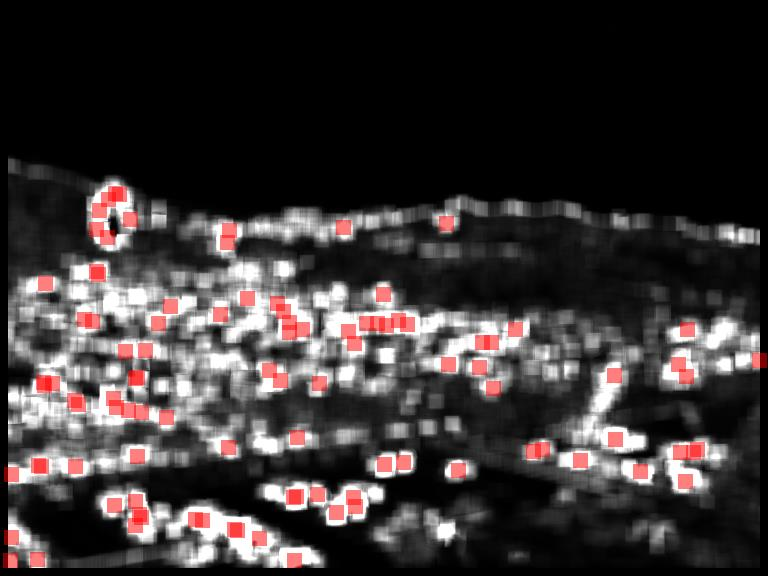
\includegraphics[scale=.6]{./img/out.jpg}

\section{考察}

今回の実験では,前回行った特徴点らしさの画像全体から,特徴的な点を選び出すプログラムを作成した.
得られた画像は,空のような色の変化が少ない場所では赤いマーカーがなく,それ以外の場所では
たくさんのマーカーが出ているので,今回実装したMatrixLocalMax関数がうまく機能しているといえる.

MatrixLocalMax関数の15x15の領域の極大値を求める処理を,2段階に分割することで
処理時間を約2分の1にすることができた.
前回は2段階に処理を分けることで30/225の処理時間短縮ができたが,前回ほどの効率化はできなかった.

前回の特徴点らしさの画像がうまく作成されない問題はコメントによる助言で解決することができた.

\end{document}
